% ---------------------------------------------------
% TSP 2016 Conference Template
% ---------------------------------------------------


\documentclass[conference,a4paper,twocolumn]{IEEEtran}

\IEEEoverridecommandlockouts


% *** GRAPHICS RELATED PACKAGES ***
%
\ifCLASSINFOpdf
\else
\fi


  \usepackage{tipa}
  \usepackage[pdftex]{graphicx}
	\usepackage{epsfig}
	\usepackage{epstopdf}


% *** MATH PACKAGES ***
%
\usepackage[cmex10]{amsmath}


% *** SUBFIGURE PACKAGES ***
\usepackage{subfigure}

\hyphenation{op-tical net-works semi-conduc-tor}

% *** CUSTOME (added by Alexander Senov) PACKAGES ***
%\usepackage[utf8x]{inputenc} % указывает кодировку документа
%\usepackage[T2A]{fontenc} % указывает внутреннюю кодировку TeX 
%\usepackage[russian,english]{babel} % указывает язык документа
%\usepackage{lmodern}
%\usepackage{gentium}
%\renewcommand*\rmdefault{phv}
\usepackage{color} % для цветного текста

\usepackage{lipsum} % for dummy text

\newcommand{\convnet}{ConvNet~} % я не знаю как правильно называть сетку в тексте, вместо этого вставляю эту команду

\newcommand{\todo}[1]{\textcolor{red}{\textbf{[#1]}}} % чтобы в глаза бросалось
% ---------------------------------------------------
% Begin of Document
% ---------------------------------------------------

\begin{document}

% ---------------------------------------------------
% Title
% ---------------------------------------------------

% Titles are generally capitalized except for words such as a, an, and, as,
% at, but, by, for, in, nor, of, on, or, the, to and up, which are usually
% not capitalized unless they are the first or last word of the title.
% Linebreaks \\ can be used within to get better formatting as desired.
% Do not put math or special symbols in the title.


\title{Arabic Manuscript Author Verification Using\\ 
Deep Convolutional Networks}

% ---------------------------------------------------
% Authors, Affiliation, and Acknowledgment
% ---------------------------------------------------



% conference papers do not typically use \thanks and this command
% is locked out in conference mode. If really needed, such as for
% the acknowledgment of grants, issue a \IEEEoverridecommandlockouts
% after \documentclass

% for over three affiliations, or if they all won't fit within the width
% of the page, use this alternative format:
% 
\author{
\IEEEauthorblockN{
Andrei Boiarov\IEEEauthorrefmark{1},
Alexander Senov\IEEEauthorrefmark{2},
Alexander Knysh\IEEEauthorrefmark{3} and
Dmitry Shalymov\IEEEauthorrefmark{4}
}
\IEEEauthorblockA{
	\IEEEauthorrefmark{1}\IEEEauthorrefmark{2}\IEEEauthorrefmark{4}
	Faculty of Mathematics and Mechanics\\
	Saint Petersburg State University\\
	Saint Petersburg, Russia\\
	Email: 
		\IEEEauthorrefmark{1}a.boiarov@spbu.ru, 
		\IEEEauthorrefmark{2}alexander.senov@gmail.com, 
		\IEEEauthorrefmark{4}dmitry.shalymov@gmail.com
}
\IEEEauthorblockA{
\IEEEauthorrefmark{3}Department of Near Eastern Studies\\
University of Michigan\\
Ann Arbor, Michigan 48104-1608, USA\\
Email: alknysh@umich.edu}
\thanks{This research is supported by Saint Petersburg State University grant 6.37.181.2014. The authors express their deep gratitude to Mrs. Evyn Kropf of the Hatcher Graduate Library who kindly facilitated access to the University of Michigan library resources.}
}

% use for special paper notices
%\IEEEspecialpapernotice{(Invited Paper)}




% make the title area
\maketitle


% ---------------------------------------------------
% Abstract
% ---------------------------------------------------

% As a general rule, do not put math, special symbols or citations
% in the abstract
\begin{abstract}
\lipsum[5]
\end{abstract}

% no keywords

% For peer review papers, you can put extra information on the cover
% page as needed:
% \ifCLASSOPTIONpeerreview
% \begin{center} \bfseries EDICS Category: 3-BBND \end{center}
% \fi
%
% For peerreview papers, this IEEEtran command inserts a page break and
% creates the second title. It will be ignored for other modes.
\IEEEpeerreviewmaketitle

% ---------------------------------------------------
% Introduction
% ---------------------------------------------------

\section{Introduction}
\label{sec:introduction}
\todo{Replace dummy text with normal}
\lipsum[6-10]
%\pagebreak
	

\begin{figure*}[!t]
	\center
  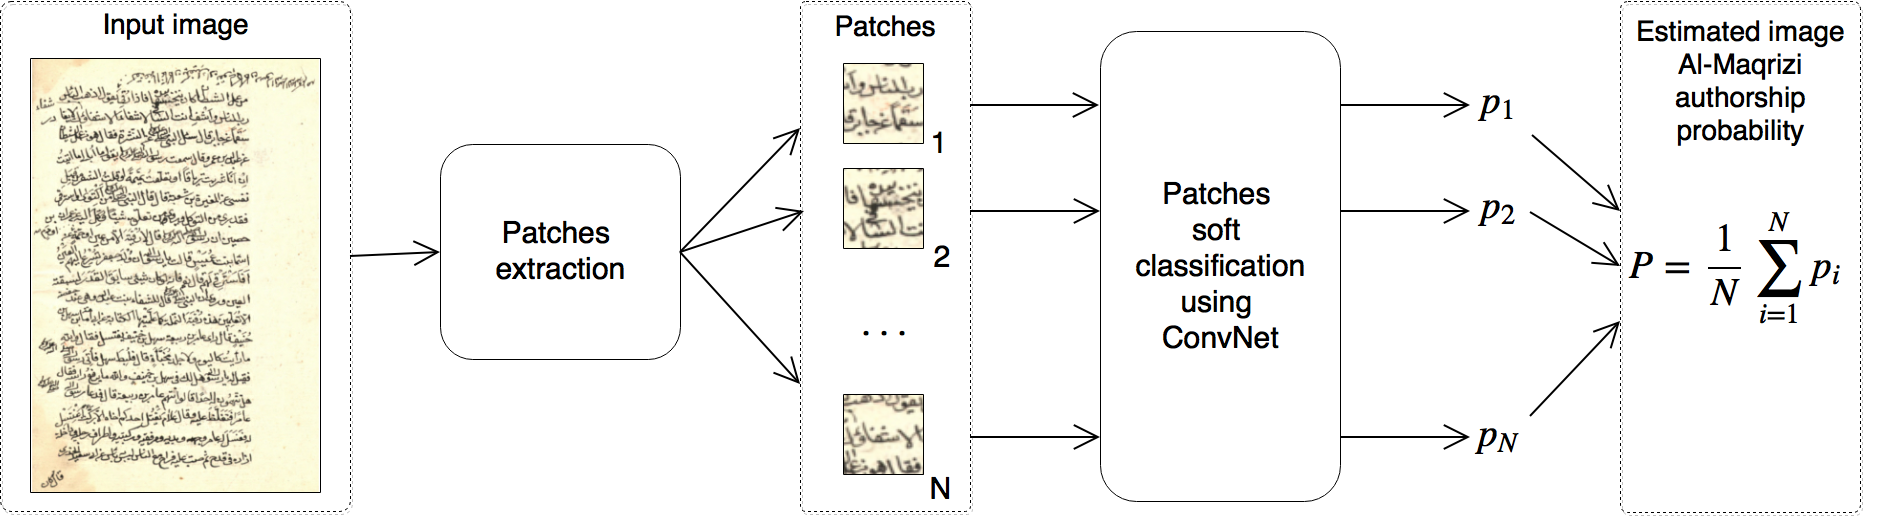
\includegraphics[width=\textwidth]{figures/Al-Maqrizi_classification_pipeline.png}
  \caption{Al-Maqrizi authorship soft classification pipeline}
  \label{fig:pipeline}
\end{figure*}	
	
\section{The Data}
\label{sec:the_data}
\todo{Replace dummy text with normal}
\lipsum[11-14]


%\pagebreak

\section{The Method}
\label{sec:the_method}

We consider author verification problem as a binary classification problem: Al-Maqrizi class denoted as $1$ and non-Al-Maqrizi class denoted as $0$. In this context our goal is to build a classification pipeline able predict the probability (\textit{soft} classification) that given image belongs to the $1$ (Al-Maqrizi) class. The entire Al-Maqrizi authorship classification pipeline illustrated at figure~\ref{fig:pipeline} consists of the following steps:

\begin{enumerate}
	\item Image preprocessing.
	\item Extracting patches from candidate image.
	\item Patches soft classification using \convnet.
	\item Averaging predicted patches probabilities to produce overall candidate image Al-Maqrizi authorship probability.
\end{enumerate}



Each of this steps are thoroughly described in the following sections.	

%The heart of our method is a \convnet patches classifier. We use ground-truth labelled patches extracted from images described in section~\ref{sec:the_data} as a training set for \convnet. [SOME DEFERRABLES FOR \convnet HERE].

\todo{Describe image preprocessing}

\subsection{Patches extraction}
The patches extraction method generates a set of sub-images called patches from given image. The basic idea is that patch should represent small but yet meaningful part of image for the main purpose - authorship verification. We use two alternative methods for patches extraction described in following subsections.

\subsubsection{Sliding window based method}
This method splits given image by a grid of fixed cell size. Each cell further used as a patch. Figure~\ref{fig:patches_example_sliding_window} \todo{add figure} illustrates the idea. 

\subsubsection{Connected components based method}
This method uses following routine for patches extraction

\begin{enumerate}
	\item Input image binarization using Otsu's filter \todo{reference to Otsu filter paper}.
	\item Connected components extraction from binarized image using algorithm from \todo{reference to connected components paper}.
c	\item Too small, too big and too stretched connected components filtering using several empirical rules \todo{specific rules description}.
	\item Outlier connected components filtering using DBSCAN \todo{reference to DBSCAN paper} clustering algorithm.
	\item Using remaining connected components bounding boxes as patches.
\end{enumerate}

Example of connected components based patches show on figure~\ref{fig:patches_example_connected components} \todo{add figure}. 

It could be seen, that connected components based patches usually consist of one or few letters thus providing high robustness for different image scale and size in contrast to fixed-size sliding window patches. However, fixed-sliding patches contain much more information: several symbols from several lines, - a very important feature for the authorship verification.



\todo{Fill this section}


\section{Results and Discussion}


\todo{Fill this section}

\section{Conclusion}


\todo{Fill this section}

% ---------------------------------------------------
% References
% ---------------------------------------------------

% can use a bibliography generated by BibTeX as a .bbl file
% BibTeX documentation can be easily obtained at:
% http://www.ctan.org/tex-archive/biblio/bibtex/contrib/doc/
% The IEEEtran BibTeX style support page is at:
% http://www.michaelshell.org/tex/ieeetran/bibtex/
%\bibliographystyle{IEEEtran}
% argument is your BibTeX string definitions and bibliography database(s)
%\bibliography{IEEEabrv,../bib/paper}
%
% <OR> manually copy in the resultant .bbl file
% set second argument of \begin to the number of references
% (used to reserve space for the reference number labels box)

\begin{thebibliography}{99}

\bibitem{MBulacu} M.~Bulacu, L.~Schomaker, A.~Brink \lq\lq Text-independent writer identification and verification on offline arabic handwriting,\rq\rq~in~\emph{Proc. 9th International Conference on Document Analysis and Recognition, ICDAR}, Curitiba, 2007, pp.~769--773.

\bibitem{DFecker} D.~Fecker, A.~Asi, W.~Pantke, V.~Märgner, J.~El-Sana, T.~Fingscheidt \lq\lq Document Writer Analysis with Rejection for Historical Arabic Manuscripts,\rq\rq~in~\emph{Proc. 14th nternational Conference on Frontiers in Handwriting Recognition, ICFHR}, Crete, 2014, pp.~743--748.

\bibitem{DL} Y.~Lecun, Y.~Bengio, G.~Hinton, \lq\lq Deep learning,\rq\rq~\emph{Nature}, no.~521, pp.~436--444, May.~2015.

\bibitem{CNN} Y.~Lecun, L.~Bottou, Y.~Bengio, P.~Haffner, \lq\lq Gradient-based learning applied to document recognition,\rq\rq~in~\emph{Proc. of the IEEE}, 1998, pp.~2278--2324.

\bibitem{Alexnet} A.~Krizhevsky,I.~Sutskever, G.~Hinton, \lq\lq ImageNet Classification with Deep Convolutional Neural Networks,\rq\rq~in~\emph{Advances in Neural Information Processing Systems}, vol.~25, 2012, pp.~1097--1105.

\bibitem{Googlenet} C.~Szegedy, W.~Liu, Y.~Jia, P.~Sermanet, S.~Reed, D.~Anguelov, D.~Erhan, V.~Vanhoucke, A.~Rabinovich, \lq\lq Going deeper with convolutions,\rq\rq~in~\emph{Proc. of the IEEE Conference on Computer Vision and Pattern Recognition}, Boston, 2015, pp.~1--9.

\bibitem{GranVolk} O.~Granichin, V.~Volkovich, D.~Toledano-Kitai, \emph{Randomized Algorithms in Automatic Control and Data Mining}. Springer-Verlag: Heidelberg, New York, Dordrecht, London, 2015, 251~p.

\end{thebibliography}

% ---------------------------------------------------
% End of Document
% ---------------------------------------------------

% that's all folks
\end{document}


